\section{Fases del flujo de trabajo en Kanban}

En el contexto de Kanban, el \textbf{flujo de trabajo} representa la secuencia de pasos o estados por los que atraviesan las tareas desde que se conciben hasta que se completan. Este flujo no es rígido, sino que se adapta a las necesidades específicas de cada equipo o proceso organizacional. El objetivo es visualizar, gestionar y optimizar el flujo para garantizar una entrega continua de valor.

\subsection{Importancia del flujo de trabajo}

La visualización del flujo permite:
\begin{itemize}
    \item Identificar cuellos de botella y retrasos.
    \item Evaluar la eficiencia del proceso actual.
    \item Establecer límites de trabajo en curso (WIP) por fase.
    \item Mejorar continuamente el rendimiento del equipo.
\end{itemize}

Además, una representación clara del flujo facilita la comprensión compartida del proceso y promueve la colaboración entre los miembros del equipo.

\subsection{Fases comunes en un tablero Kanban}

Si bien cada implementación de Kanban puede diferir, muchas organizaciones adoptan una estructura de flujo que comprende las siguientes etapas:

\subsubsection{Backlog / Ideas / Por hacer (\textit{To Do})}

En esta fase se encuentran todas las tareas aún no iniciadas. Representa el conjunto de elementos que están listos para ser priorizados y ejecutados. Es habitual que se realicen sesiones de refinamiento para evaluar la viabilidad, esfuerzo requerido y prioridad de estas tareas.

\subsubsection{En progreso (\textit{Doing})}

Corresponde a las tareas que se encuentran activamente en desarrollo. Este estado refleja el trabajo que está siendo ejecutado por los miembros del equipo. Es recomendable que cada miembro se enfoque en una o pocas tareas a la vez para evitar la sobrecarga de trabajo y fomentar la finalización efectiva.

\subsubsection{Revisión / Pruebas / Validación}

Una vez completado el desarrollo inicial de una tarea, esta puede requerir validaciones adicionales. Dependiendo del tipo de proyecto, esta fase puede incluir:
\begin{itemize}
    \item Revisión de código
    \item Pruebas funcionales o de integración
    \item Verificación del cumplimiento de criterios de aceptación
    \item Evaluación por parte del cliente o partes interesadas
\end{itemize}

Esta etapa asegura la calidad antes de dar por finalizada la entrega.

\subsubsection{Hecho (\textit{Done})}

Representa la finalización formal de una tarea. Las tareas en esta columna han sido revisadas, validadas y están listas para su despliegue o ya han sido entregadas al cliente. Este estado implica cumplimiento total de los requisitos establecidos.

\subsection{Ejemplo de flujo de trabajo adaptado}

En un entorno de desarrollo de software, el flujo de trabajo podría incluir fases adicionales como:
\begin{itemize}
    \item Diseño UI/UX
    \item Aprobación del Product Owner
    \item Despliegue a producción
\end{itemize}

Por otro lado, en equipos de atención al cliente o marketing, las fases pueden ser completamente diferentes. Lo esencial es que el flujo refleje de forma precisa cómo se ejecuta el trabajo en el contexto real del equipo.

\subsection{Visualización de un flujo de trabajo típico}

\begin{figure}[H]
\centering
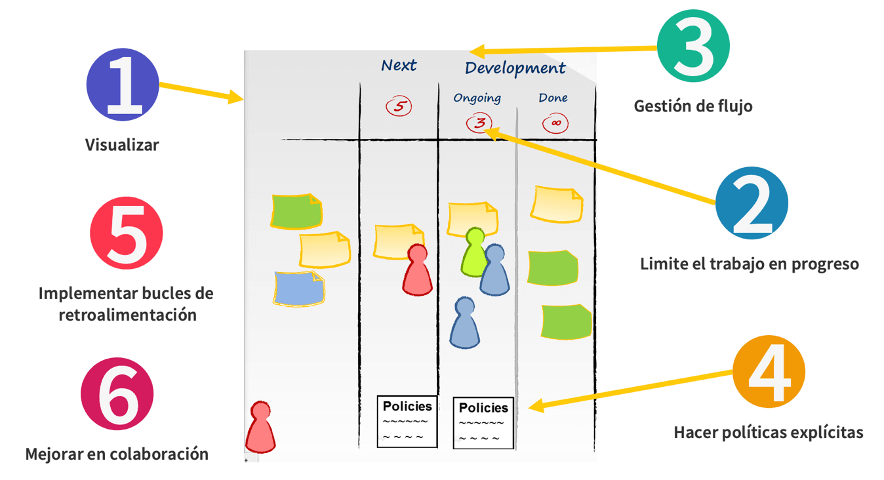
\includegraphics[width=0.9\textwidth]{assets/images/flujo-kanban.png}
\caption{Ejemplo de un flujo de trabajo típico en un tablero Kanban.}
\end{figure}

Este ejemplo gráfico evidencia cómo se puede estructurar visualmente el recorrido de una tarea desde su planificación hasta su finalización.

\subsection{Consideraciones sobre la personalización del flujo}

Kanban no prescribe fases específicas ni impone un modelo único. De hecho, uno de sus principios fundamentales es adaptarse al flujo actual y evolucionarlo progresivamente. Esto significa que:
\begin{itemize}
    \item Cada equipo puede definir su propio flujo de trabajo.
    \item Las fases pueden cambiar con el tiempo conforme se detectan oportunidades de mejora.
    \item Se deben documentar y comunicar las políticas que regulan la transición entre fases.
\end{itemize}

La capacidad de adaptación es uno de los factores clave que diferencian a Kanban de otras metodologías ágiles más prescriptivas.

